% !TEX root =  ../main.tex

McMinn~\cite{McMinn2004} defined search-based software testing (SBST) as \textit{``using a meta-heuristic optimizing search technique, such as a genetic algorithm, to automate or partially automate a testing task"}.
Within this realm, test data generation at different testing levels (such as \textit{unit testing}, \textit{integration testing}, \etc) has been actively investigated~\cite{McMinn2004}. This section 
provides an overview of earlier work in this area.


%As it defined by McMinn \cite{McMinn2011}, \textit{"Search-Based Software Testing is the use of a meta-heuristic optimizing search technique, such as a Genetic Algorithm, to automate or partially automate a testing task"}.
%Among these tasks, test data generation in different testing levels (such as \textit{unit testing}, \textit{integration testing}, \etc) is one of the most contributed ones \cite{McMinn2004}.
%This section outlines a summary of the previous studies about applying search-based test data generation in various levels.

\subsection{Search-based approaches for unit testing}
SBST algorithms have been extensively used for unit test generation. Previous studies confirmed that thus generated tests achieve a high code coverage~\cite{Panichella2018a, Campos2018}, real-bug detection~\cite{almasi2017industrial}, and debugging cost reduction~\cite{soltani2017, Panichella2016}, complementing manually-written tests.


From McMinn's \cite{McMinn2004} survey about search-based test data generation, we observe that most of the current approaches rely on the control flow graph (CFG) to 
abstract the source code and represent possible execution flows. The $CFG_m=(N_m,E_m)$ represents a method\footnote{Or function in procedural programming languages.} $m$ as a directed graph of \textbf{basic blocks} of code (the nodes $N_m$), while $E_m$ is the set of the control flow edges. An edge connects a basic block $n_1$ to another one $n_2$ if the control may flow from the last statement of $n_1$ to the first statement of $n_2$.

%Following McMinn \etal's \cite{McMinn2004} survey about search-based test data generation, one of the widely used categories of approaches for automating this task is structural-based generation. These approaches use a control flow graph (CFG) to abstract the source code and represent possible execution flows.
%The \textit{control flow graph (CFG)} of method $m$ is a directed graph $CFG_m=(N_m,E_m)$ representing all paths that might be traversed through the method. In this graph, $N_m$ is the set of the \textit{basic blocks} in method $m$, and $E_m$ is the set of the control flow edges.
%A \textit{basic block} is a maximum sequence of non-branching statements in a
%method having only one entry point and one exit point.
%If one of the statements of a basic block is executed, other statements in this
%block are executed as well.
%In a CFG, an edge connects a basic block $n_1$ to another one $n_2$ if the control may flow from the last statement of $n_1$ to the first statement of $n_2$.

Listing~\ref{list:cling:ClassA} presents the source code of \texttt{Person}, a class representing a person and her transportation habits. A \texttt{Person} can drive home (lines 4-10), or add energy to her car (lines 12-18). The right-hand side of Figure~\ref{fig:cling:CCFG} presents the CFG of two of Person's methods, with the labels of the nodes representing the line numbers in the code. Since method \texttt{driveToHome} calls method \texttt{addEnergy}, \texttt{node 6} is transformed to two nodes, which are connected to the entry and exit point of the called method. This transformation is explained in the last paragraph of this section. 

\begin{lstlisting}[frame=tb,
    caption={Class \texttt{Person}},
    label=list:cling:ClassA,
    language=java,
    captionpos=t,
    numbers=left,
    belowskip=-2.5em,
    float=t,
    firstnumber=1]
class Person{
    private Car car = new Car();
    protected boolean lazy = false;
    public void driveToHome(){
        if (car.fuelAmount < 100) {
            addEnergy();
        } else {
            car.drive();
        }   
    }

    protected void addEnergy(){
        if (this.lazy) {
            takeBus();
        } else {
            car.refuel();
        }
    }   
    }
  \end{lstlisting}
%   \captionof{codetype}{Type definitions}
  
 
%  \begin{figure*}[htb]
%    
%    \centering % <-- added
%\begin{subfigure}{0.25\textwidth}
%  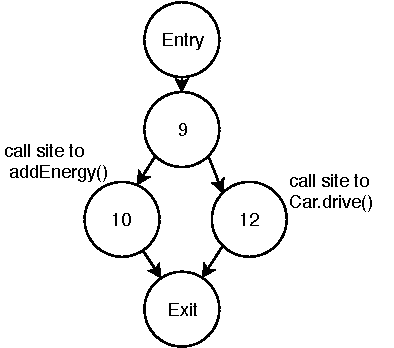
\includegraphics[width=\linewidth]{figures/driveToHome}
%  \caption{CFG of Person.driveToHome()}
%  \label{fig:driveToHome}
%\end{subfigure}\hfil % <-- added
%\begin{subfigure}{0.25\textwidth}
%  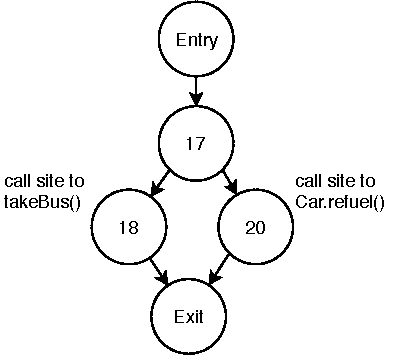
\includegraphics[width=\linewidth]{figures/refuelCar}
%  \caption{CFG of Person.addEnergy()}
%  \label{fig:refuelCar}
%\end{subfigure}\hfil % <-- added
%\begin{subfigure}{0.25\textwidth}
%  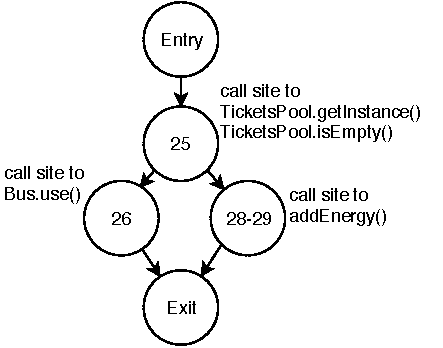
\includegraphics[width=\linewidth]{figures/takeBus}
%  \caption{CFG of Person.takeBus()}
%  \label{fig:takeBus}
%\end{subfigure}
%\caption{CFGs of methods in class $Person$}
%\label{fig:personClass}
%\end{figure*}





Many structural-based approaches combine two common heuristics to reach a high branch and statement coverage in unit-level testing. These two heuristics  are \textit{approach level} and \textit{branch distance}.
The \textit{branch distance} measures (based on a set of rules) the distance to \textit{satisfying} (true branch) and the distance to \textit{not satisfying} (false branch) a particular branching node in the program.
The \textit{approach level} measures the distance between the execution path and a target node in a CFG. To describe how this heuristic measures this distance, we 
rely on the concepts of \textbf{post-dominance} and \textbf{control dependency}~\cite{Allen:1970:CFA:800028.808479}.
%
%need to describe \textit{post-domination} and \textit{control dependency} first. Node $y$ in a CFG \textit{post-dominates} node $x$ if and only if every path from $x$ to the exit point of CFG contains $y$. Node $z$ in a CFG \textit{post-dominates} an edge $(x,y)$ if and only if every path from $x$ to the exit point through $(x,y)$ passes by $z$. Finally, node $y$ in a CFG is \textit{control dependent} on $x$ if $y$ post dominates one of the outgoing edges of $x$, but it does not pos-dominate node $x$ itself. 
%
As an example, in Figure \ref{fig:cling:CCFG}, \textit{node 8} is control dependent on \textit{node 5} and \textit{node 8} post-dominates edge $\langle 5,8\rangle$. %, but it does not post-dominate $node 5$ itself ($node 5$ can reach the exit point through $node 6$). 
The \textit{approach level} is the minimum number of control dependencies between a target node and an executed path by a test case. 

% \medskip
In search-based unit testing, each generated test case is a sequence of method calls to a target class. This call sequence can be generated randomly, or it can be generated using existing resources. Goffi \etal \cite{Goffi2016} leverage existing documentation in this process, but for various reasons it does not allow to detect all bugs~\cite{robillard2011,blasi2018,zhou2017}.
%introduce a tool called Toradocu, which can be integrated into the test data generation process to leverage the existing documentation of the target class in this process. They show that this approach helps the test generation process to detect more exceptional bugs. However, since documentation is incomplete \cite{robillard2011}, outdated \cite{blasi2018}, or defective \cite{zhou2017}, it is not sufficient for detecting all of the bugs.
Rojas \etal~\cite{Rojas2016} collect the usages of classes in the existing test cases to generate the call sequences. To reach that goal, they need to execute each of the existing tests to find the call sequences; this may be a time taking process.

In this study, we analyze how a class is used/invoked by the other classes. For this purpose, we merge the Class-level Control Flow Graph (CCFG) of target callee and caller classes. 


% which enriches the CFG with the calls (edges) between a target callee class and a caller class (represented using dashed lines in Figure \ref{fig:CCFG}). The CCFG is the main source we will use to generate integration tests between these two classes.


\subsection{Search-based approaches for integration testing}

Integration testing aims at finding faults that are related to the interaction between components.
We discuss existing integration testing criteria and explain the search-based approaches that use these criteria to define fitness functions for automating integration-level testing tasks.

\subsubsection{Integration testing criteria}
\label{sec:background-integ-testing-criteria}

\begin{figure}[t]
    \centering
	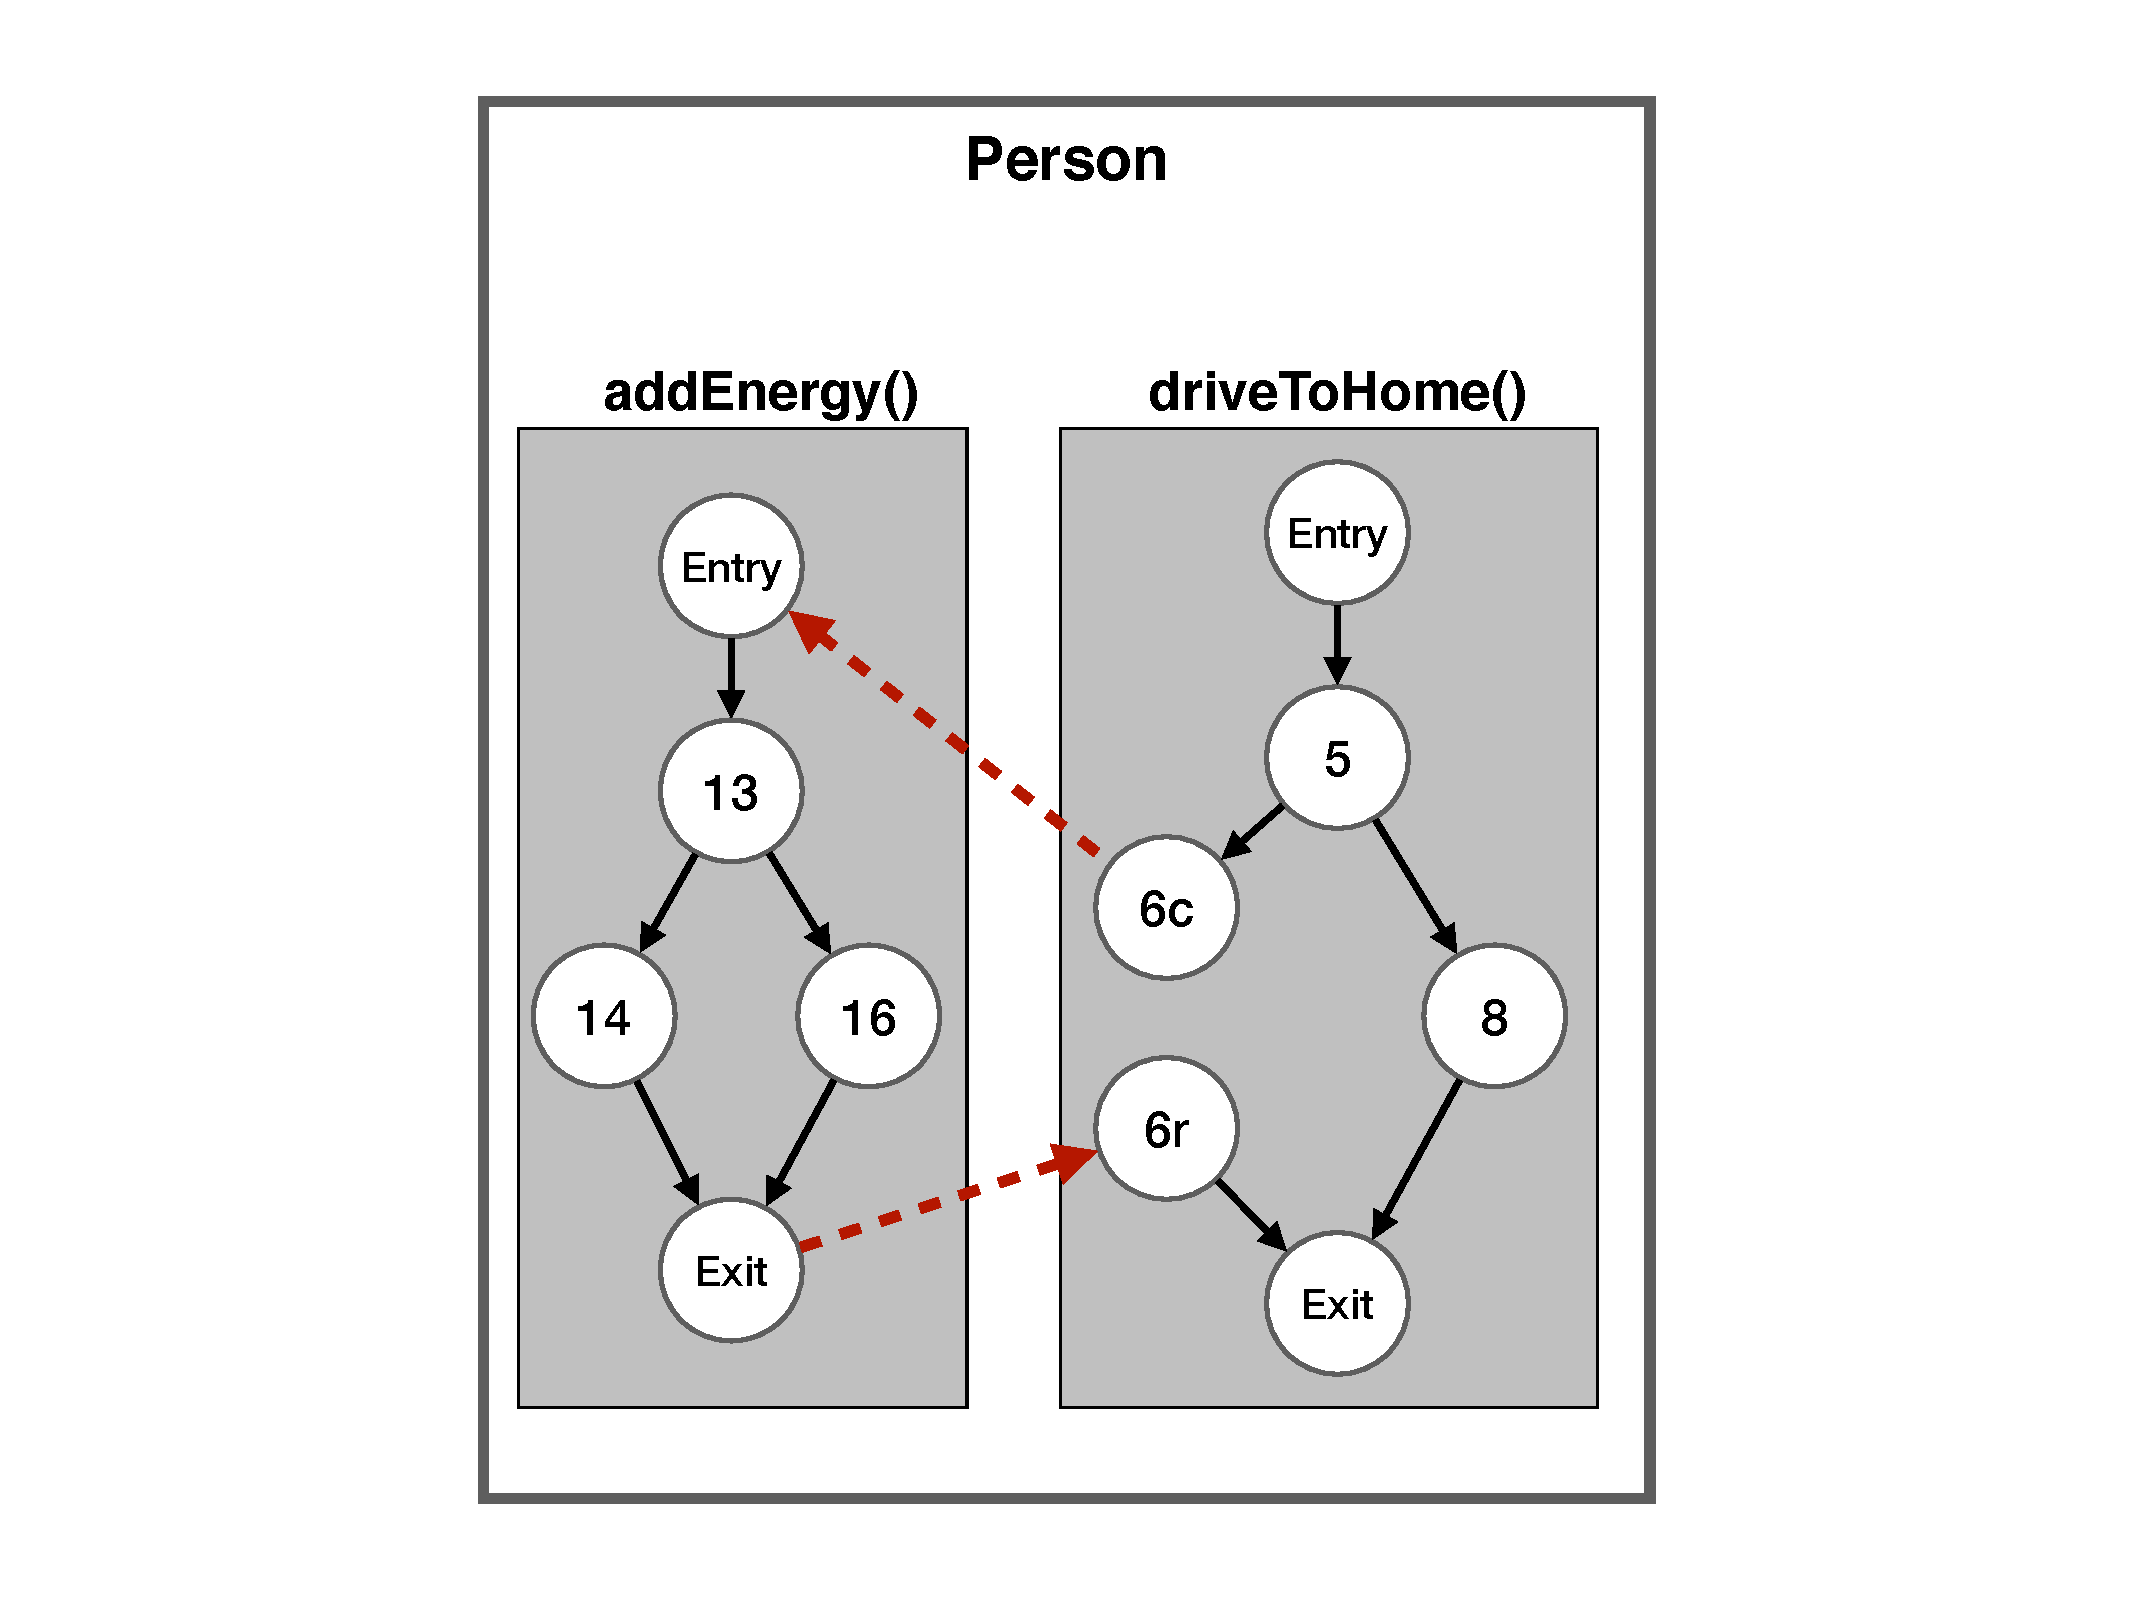
\includegraphics[width=0.85\linewidth]{papers/cling/figures/CCFG_new}
	\caption{Class-level CFG for class \texttt{Person}}
  \label{fig:cling:CCFG}
\end{figure}


 Jin \etal \cite{Jin1998} categorize the connections between two procedures into four levels for testing: \textit{call couplings} (level 1) occur when one procedure calls another procedure; \textit{parameter couplings} (level 2) happen when a procedure passes a parameter to another procedure; \textit{shared data couplings} (level 3) occur when two procedures refer to the same data objects; \textit{external device coupling} (level 4) happens when two procedures access the same storage device.
They introduce integration testing criteria according to the data flow graph (containing the definitions and usages of variables at the integration points) of procedure-based software. Their criteria, called \textit{coupling-based testing criteria}, require that the developed tests execute paths in the CFG of a procedure (the \textit{caller procedure}) which starts from the definition of a variable to a node (the \textit{call site}) which calls another procedure.
%The defined integration testing criteria are transformed to adapt to the object-oriented paradigm. 
%By moving from procedural-based programming to object-oriented programming, the defined integration testing criteria are transformed to adapt to this type of programming. 

Harrold \etal \cite{Harrold1994} introduced data flow testing for a single class focusing on method-integration testing. They define three levels of testing: \textit{intra-method testing}, which tests an individual method (\ie the smallest possible unit to test); \textit{inter-method testing}, in which a public method is tested that (in)directly calls other methods of the same class, and \textit{intra-class testing}, in which the various sequences of public methods in a class are tested. For data flow testing of inter-method and intra-class testing, they defined a \textit{Class-level Control Flow Graph} (CCFG). The CCFG of class \textit{C} is a directed graph $CCFG_C=(N_{Cm},E_{Cm})$ which is a composition of the control flow graphs of methods in $C$; the CFGs are connected through their call sites to methods in the same class~\cite{Harrold1994}. This graph demonstrates all paths that might be crossed within the class by calling its methods or constructors. 


Let us consider again the class $Person$ in Listing~\ref{list:cling:ClassA}. The CCFG of class $Person$ is created by merging the CFGs of its method, as demonstrated in Figure~\ref{fig:CCFF_new}.
For example, in the CFG of the method \texttt{Person.driveToHome()}, the \textit{node 6c} is a call site to \texttt{Person.addEnergy()}. In the approach introduced by Harrold \etal \cite{Harrold1994}, they detect the def-use paths in the constructed CCFGs and try to cover those paths.
%The CCFG of a class is created by merging the CFGs of methods in this class. Following Harrold \etal's \cite{Harrold1994} approach, the first step for creating CCFG is finding all of the call sites to the methods in the same class. Next, we replace these call sites with a \emph{call node} and a \emph{return node}. Finally, we add one edge from the \emph{call node} to the entry node of the called method, and onther edges from the exit nodes of the called method to the \emph{return node}.

%\begin{figure*}[htb]
%    \centering % <-- added
%
%\begin{subfigure}{0.3\textwidth}
%    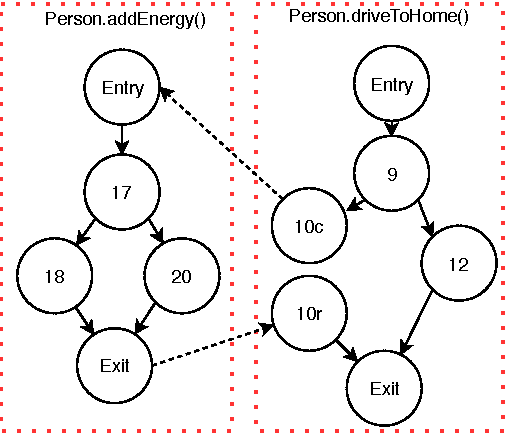
\includegraphics[width=\linewidth]{figures/merge-two-CFGs}
%    \caption{Merging methods driveToHome() and addEnergy()}
%    \label{fig:cfg-merge}
%  \end{subfigure}
%  \begin{subfigure}{0.5\textwidth}
%    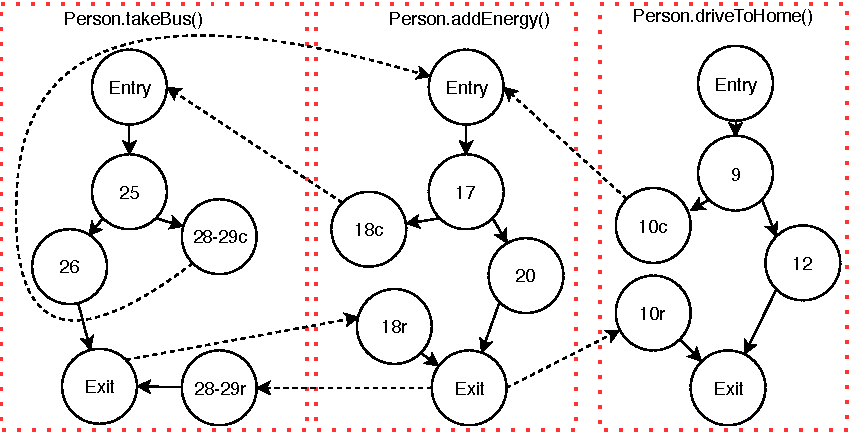
\includegraphics[width=\linewidth]{figures/ACCFG}
%    \caption{Class control flow graph of A}
%    \label{fig:accfg}
%  \end{subfigure}
%
%\caption{Creating  class control flow graph of class Person}
%\label{fig:images}
%\end{figure*}



%Figure~\ref{fig:cfg-merge} shows the result of this merging of two CFGs. 
%When we merge all of the CFGs of the class $Person$, the final CCFG is shown in Figure~\ref{fig:accfg}.

A special case is represented by the polymorphic interactions that need to be tested. Alexander \etal \cite{Alexander2000, Alexander2003, Alexander2004,Alexander2010} used the data flow graph to define testing criteria for integrations between classes in the same hierarchy tree.
 %Moreover, they showed that the introduced criteria are more efficient at detecting faults than branch coverage \cite{Alexander2002a}.

 All of the mentioned approaches are using data-flow graphs to define integration testing criteria. However, generating data-flow graphs covering the def-uses involved in between classes is expensive and not scalable in complex cases. Vivanti \etal \cite{vivanti2013search} shows that the average number of def-use paths in a single class in isolation is three times more than the number of branches. By adding def-use paths between the non-trivial classes, this number grows exponentially.
 In our approach, since the number of search objectives matters (\ie too many objectives leads to the search process misguidance), we do not try to cover def-use paths. 

 Alternatively, we merge the CCFG of two classes (caller and callee class) to apply \textbf{class integration testing}. As an example, Figure \ref{fig:CCFF_new} merges two classes by linking their CFGs.
 This type of graphs is used previously for other usages. For instance, Wang \etal \cite{wang2019could} merge the CFGs of methods of classes in the dependencies of software under test to identify the dependency conflicts.
We use these merged graphs to define a new class integration testing criterion, which focuses on covering different branches in both of the classes. Our approach also considers special cases of interaction, namely inheritance and polymorphism. 


% However, in this study, we will use the CCFG of two classes to apply \textbf{class integration testing}.
\subsubsection{Search-based approaches}

Search-based approaches are widely used for test ordering \cite{Wang2010, Steindl2012, Hashim2005, Vergilio2012, Bansal2009, JIiang2019, Borner2009, Mariani2016, Guizzo2015, Abdurazik2009, DaVeigaCabral2010, Briand2003a, Vergilio2012}, typically with the aim of executing those tests with the highest likelihood of failing earlier on. % These studies propose a solution for ordering the integration testing of the classes in the software under test (SUT). However, they do not offer any solution for automated integration test generation.
However, search-based approaches have rarely been used for generating integration tests. Ali Khan \etal \cite{AliKhan2013} have proposed a high-level evolutionary approach that detects the coupling paths in the data-flow graphs of classes and have used it to define the fitness function for the genetic algorithm. Then, the fitness function aids the genetic algorithm to generate tests for the detected coupling paths. Moreover, they proposed another approach for the same goal, which uses Particle Swarm Optimization \cite{Khan2014}. However, The paper does not describe the fitness function and genetic algorithm used in their approach, nor any evaluation for examining the quality of the tests generated by this approach. 
The paper also does not check whether the tests can complement tests generated by existing search-based unit testing approaches. Besides, since objectives are defined according to the def-use paths between classes, the number of search objectives can grow exponentially, thus severely limiting the scalability of the approach (as we explained in Section \ref{sec:background-integ-testing-criteria}).

In this study, we propose a novel approach for class integration test generation.
Instead of using the data flow graph, which is relatively expensive to construct as it needs to find the coupling paths, we use the information available in the class call graph of the classes to calculate the fitness of the generated tests. Also, we assess our generated tests using different metrics.

\subsection{Search-based approaches for other testing levels}

Arcuri \cite{Arcuri2019} proposed EvoMaster, an evolutionary-based white-box approach for system-level test generation for RESTful APIs. A test for a RESTful web service is a sequence of HTTP requests. EvoMaster tries to cover three types of targets:
 \begin{inparaenum}[(i)]
 \item all of the statements in the System Under Test (SUT);
 \item all of the branches in the SUT; and
\item different returned HTTP status codes.
\end{inparaenum}
Although EvoMaster tests different classes in the SUT, it does not systematically target different integration scenarios between classes.

In contrast to EvoMaster, other approaches perform fuzzing \cite{Holler2012}, \textit{``an automated technique providing random data as input to a software system in the hope to expose a vulnerability.''} Fuzzing uses information like grammar specifications \cite{Holler2012, beyene2012, coppit2005, godefroid2008} or feedback from the program during the execution of tests \cite{Padhye2019} to steer the test generation process.
These approaches are black-box and do not rely on any knowledge about classes in the SUT. Hence, their search processes are not guided by the integration of classes.

Our approach performs white-box testing. It monitors the interaction between the target classes and strives to cover different integration scenarios between them.
